\let\negmedspace\undefined
\let\negthickspace\undefined
\documentclass[journal]{IEEEtran}
\usepackage[a4paper, margin=10mm, onecolumn]{geometry}
%\usepackage{lmodern} % Ensure lmodern is loaded for pdflatex
\usepackage{tfrupee} % Include tfrupee package

\setlength{\headheight}{1cm} % Set the height of the header box
\setlength{\headsep}{0mm}  % Set the distance between the header box and the top of the text

\usepackage{gvv-book}
\usepackage{gvv}
\usepackage{cite}
\usepackage{amsmath,amssymb,amsfonts,amsthm}
\usepackage{algorithmic}
\usepackage{graphicx}
\usepackage{float}
\usepackage{textcomp}
\usepackage{xcolor}
\usepackage{txfonts}
\usepackage{listings}
\usepackage{enumitem}
\usepackage{mathtools}
\usepackage{gensymb}
\usepackage{comment}
\usepackage[breaklinks=true]{hyperref}
\usepackage{tkz-euclide} 
\usepackage{listings}
% \usepackage{gvv}                                        
\def\inputGnumericTable{}                                 
\usepackage[latin1]{inputenc}                                
\usepackage{color}                                            
\usepackage{array}                                            
\usepackage{longtable}                                       
\usepackage{calc}                                             
\usepackage{multirow}                                         
\usepackage{hhline}                                           
\usepackage{ifthen}                                           
\usepackage{lscape}
\usepackage{tikz}
\usetikzlibrary{patterns}

\begin{document}

\bibliographystyle{IEEEtran}
\vspace{3cm}

\title{4.3.54}
\author{ee25btech11063-vejith}

\maketitle
% \maketitle
% \newpage
% \bigskip
{\let\newpage\relax\maketitle}
\renewcommand{\thefigure}{\theenumi}
\renewcommand{\thetable}{\theenumi}
\setlength{\intextsep}{10pt} % Space between text and floats
\textbf{Question}\\
A line is such that its segment between the lines 5x-y+4=0 and 3x+4y-4=0 is bisected at the point (1,5).obtain its equation\\
\textbf{Solution}:\\
Given two lines are
\begin{align}
    \brak{5\hspace{0.5cm}-1}\myvec{x\\y}=-4\\
    \brak{3\hspace{0.5cm}4}\myvec{x\\y}=4
\end{align}
Let $\Vec{A}$ be the point of intersection of desired line and (1)
\begin{align}
    \Vec{A}=\myvec{x_1\\y_1}\\
    \implies \brak{5\hspace{0.5cm}-1}\myvec{x_1\\y_1}=-4\\
    \implies 5x_1-y_1=-4
\end{align}
Let $\Vec{B}$ be the point of intersection of desired line and (2)
\begin{align}
    \Vec{B}=\myvec{x_2\\y_2}\\
    \implies \brak{3\hspace{0.5cm}4}\myvec{x_2\\y_2}=4\\
    \implies 3x_2+4y_2=4
\end{align}
The mid point of $\Vec{A}$ and $\Vec{B}$ is $\myvec{1\\5}$
\begin{align}
  \frac{\Vec{A}+\Vec{B}}{2}=\myvec{1\\5}\\
  \implies \myvec{x_1\\y_1}+\myvec{x_2\\y_2}=\myvec{2\\10}\\
  \implies x_1+x_2=2\\
  \implies y_1+y_2=10
\end{align}
The equations (5),(8),(11),(12) can be written as
\begin{align}
    \begin{pmatrix}
        5 & -1 & 0 & 0\\
        0 & 0 & 3 & 4\\
        1 & 0 & 1 & 0\\
        0 & 1 & 0 & 1
    \end{pmatrix} \myvec{x_1\\x_2\\y_1\\y_2}=\myvec{-4\\4\\2\\10}\\
\end{align}
Forming the Augmented matrix,
\begin{align}
\left(\begin{array}{cccc|c}
        5 & -1 & 0 & 0 & -4\\
        0 & 0 & 3 & 4 & 4\\
        1 & 0 & 1 & 0 & 2\\
        0 & 1 & 0 & 1 & 10
\end{array}\right) &\xrightarrow{R_1 \leftrightarrow R_3} \left(\begin{array}{cccc|c}
        1 & 0 & 1 & 0 & 2\\
        0 & 0 & 3 & 4 & 4\\
        5 & -1 & 0 & 0 & -4\\
        0 & 1 & 0 & 1 & 10
\end{array}\right)\\
 &\xrightarrow{R_3 \rightarrow R_3-5R_1} \left(\begin{array}{cccc|c}
        1 & 0 & 1 & 0 & 2\\
        0 & 0 & 3 & 4 & 4\\
        0 & -1 & -5 & 0 & -14\\
        0 & 1 & 0 & 1 & 10
\end{array}\right)\\
 &\xrightarrow{R_2 \leftrightarrow R_4} \left(\begin{array}{cccc|c}
        1 & 0 & 1 & 0 & 2\\
        0 & 1 & 0 & 1 & 10\\
        0 & -1 & -5 & 0 & -14\\
        0 & 0 & 3 & 4 & 4
\end{array}\right)\\
\end{align}
\begin{align}
&\xrightarrow{R_3 \rightarrow R_3+R_2} \left(\begin{array}{cccc|c}
        1 & 0 & 1 & 0 & 2\\
        0 & 1 & 0 & 1 & 10\\
        0 & 0 & -5 & 1 & -4\\
        0 & 0 & 3 & 4 & 4
\end{array}\right)\\
&\xrightarrow{R_4 \rightarrow R_4+\frac{3}{5}R_3} \left(\begin{array}{cccc|c}
        1 & 0 & 1 & 0 & 2\\
        0 & 1 & 0 & 1 & 10\\
        0 & 0 & -5 & 1 & -4\\
        0 & 0 & 0 & 23/5 & 8/5
\end{array}\right)
\end{align}
on back substitution we get
\begin{align}
\myvec{x_1\\x_2\\y_1\\y_2}=\myvec{26/23\\222/23\\20/23\\8/23}\\
  \implies \Vec{A}=\myvec{26/23\\ 222/23}\\
\implies   \Vec{B}=\myvec{20/23 \\ 8/23}
\end{align}
Equation of a line is given by
\begin{align}
    \Vec{n}^T\Vec{x}=c.\\
    \Vec{n}=\myvec{107\\-3}\\
    \implies \brak{107\hspace{0.5cm}-3}\myvec{x\\y}=c.
\end{align}
The point $\myvec{1\\5}$ lies on the above line
\begin{align}
 \implies \brak{107\hspace{0.5cm}-3}\myvec{1\\5}=c.\\
 \implies c=92
\end{align}
The desired line is 
\begin{align}
    \brak{107\hspace{0.5cm}-3}\myvec{x\\y}=92.
\end{align}

\begin{figure}[H]
    \centering
    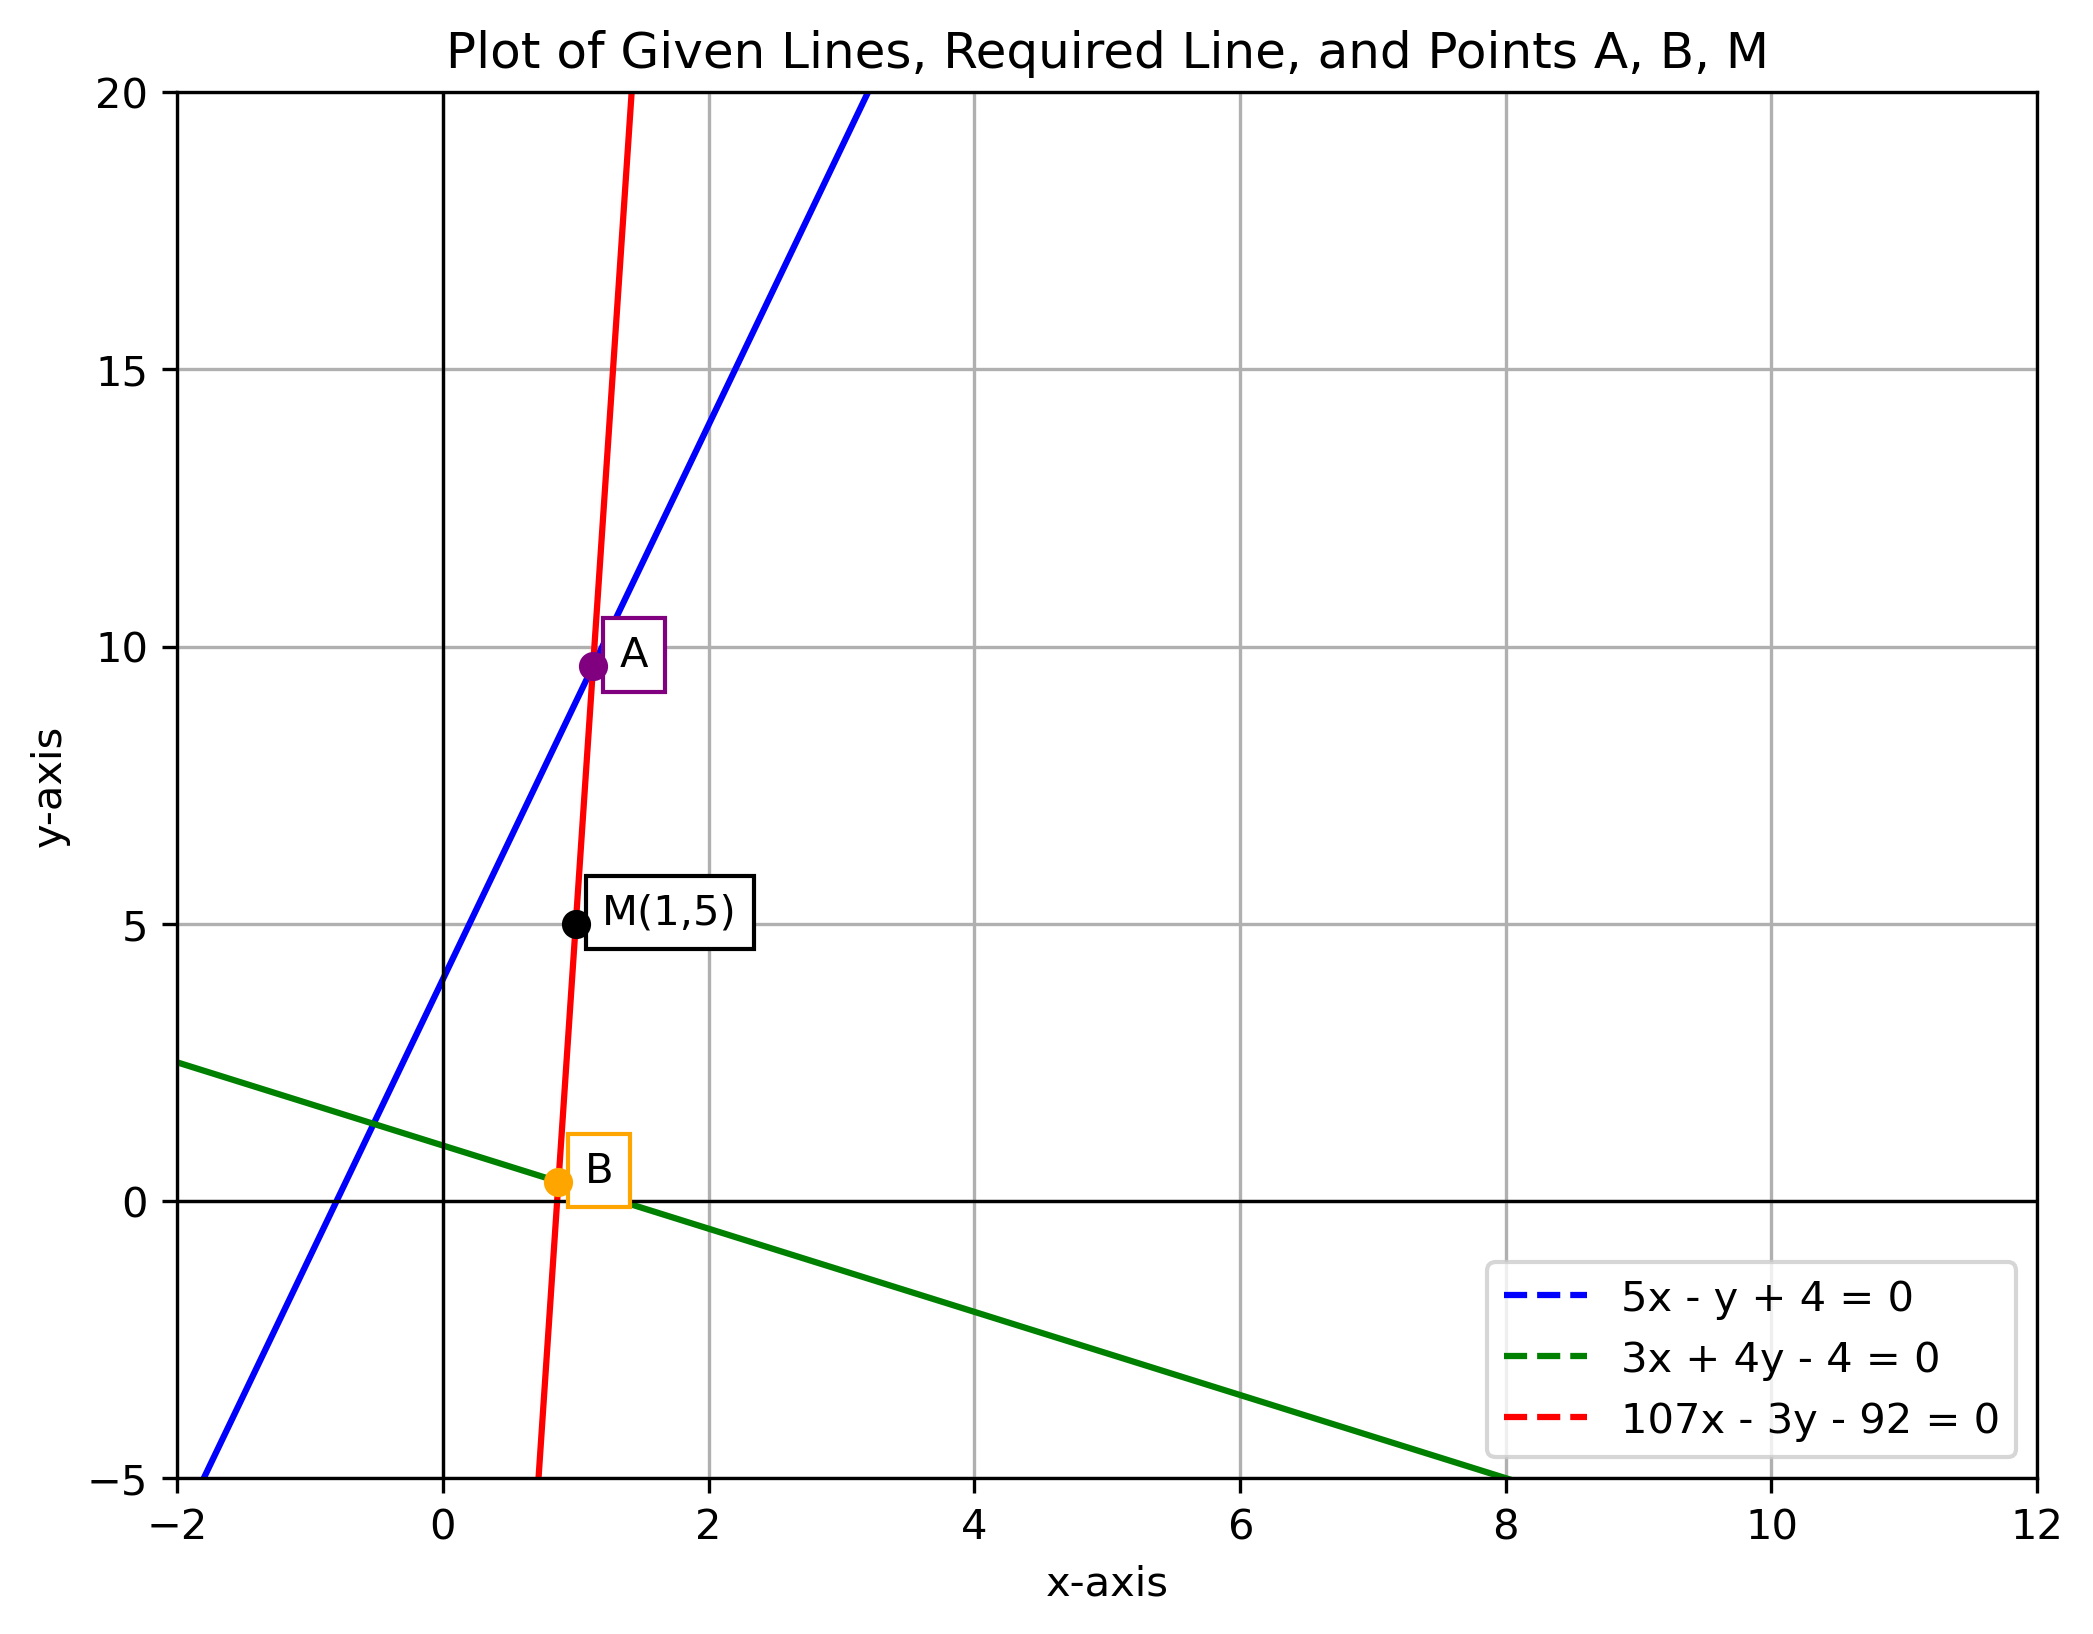
\includegraphics[width=0.7\columnwidth]{figs/01.png}
    \caption{Caption}
    \label{fig:placeholder}
\end{figure}

\end{document}
